

\section{Quick Theory}
\subsection{Digital Circuits}
Talking of circuits, we differ between analogue circuits and digital circuits. The difference lays actually in the format of the signal that represents the carried information. \newline
An analogue signal uses some attribute of the medium to convey the signal's information. In electric circuits is it the voltage, current or frequency, that is varied in order to create an electric signal. Analog electronic circuits are those in which the threshold of the current or voltage varies \underline{continuously} over time, corresponding to the information being represented. They follow Kirchhoff's circuit laws: all the currents at a node (a place where wires meet), and the voltage around a closed loop of wires is zero. \newline
In digital electronic circuits, electric signals take on \underline{discrete values} to represent logical and numeric values, which then represent the information that is being processed. Every digital circuit is also a analog circuit, but it has ideally (just two) discrete potential levels in use. 

\subsection{Binary Numbers}
%erkläre mehr, über Dezimalzahlsystem, Vergleich Dezimal/Binär, Übertrag, etc.!!! Motivation, wir haben nur zwei Zustände. 
As motivated before, we want to work with two states only, because then it is easy to make calculations. Therefore, almost always, binary encoding is used: one voltage level represents a binary '1' and another voltage, usually a value near the ground potential, represents a binary '0'. Those binary digits, each of them called one 'bit', can then be used to represent numbers and characters and therefore to carry information. The binary code was invented and first used by Gottfried Leibniz already in 1679. Back then it was more some kind of beautiful game for him to represent and deal with numbers as ones and zeros, rather than something that one could really use.

\begin{figure}[H]
\centering
\begin{minipage}{0.5\textwidth}
%  \centering
  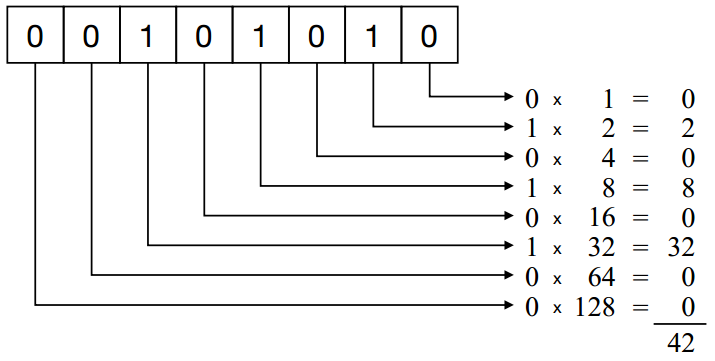
\includegraphics[width=1\textwidth]{binary.png}%
  \caption{Binary representation of one bit}%
  \label{fig:binary}
\end{minipage}%
\begin{minipage}{.4\textwidth}
  \centering
  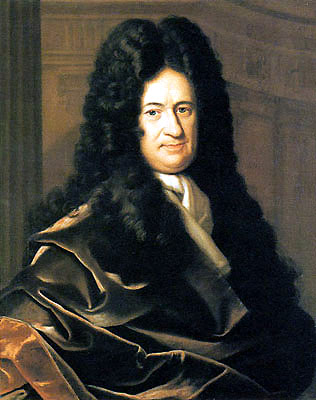
\includegraphics[width=0.8\textwidth]{leibniz}%
  \caption{Painting of Gottfried Leibniz}%
  \label{fig:leibniz}
\end{minipage}
\end{figure}

\subsection{Boolean Algebra and its implementation}
To understand how a processor can actually perform calculations and follow algorithms with those binary numbers, some knowledge about Boolean logic has to be obtained first. The Boolean Algebra (first half of the 19. century by George Boole) defines three main operations: 

%\noindent
\begin{itemize}
 \item \textbf{The conjunction:} $a\land b$ is $1$ if and only if $a$ is $1$ and $b$ is $1$.\\
 \item \textbf{The disjunction:} $a\lor b$  is $1$ if and only if $a$ is $1$ or $b$ is $1$ or $a\wedge b$ is $1$.\\
 \item \textbf{The negation:}  $\neg a$ is $1$ if and only if $a$ is $0$. A negated variable $a$ is also often written as $\overline{a}$.
\end{itemize}

\noindent
The operations of the Boolean Algebra are Associative, Commutative and Distributive. They have a Neutral, an Inverse and a Zero element. One can easily imagine, that those operations can be combined and added in number to create more complex calculation operators. This is actually exactly what happens in our computers, servers and smartphones, of course on a very large scale. 
\subsection{Truth tables}
These Boolean operators can be represented in so called truth tables as follows:

%%include also ==, XOR, etc... 

\begin{table}[H]
\centering
\begin{tabular}{c|c|c|c|c}
\textbf{$a$} & \textbf{$b$} & \textbf{$a\land b$} & \textbf{$a\lor b$} & \textbf{$\neg a$} \\ \hline
0          & 0          & 0            & 0            & 1           \\
1          & 0          & 0            & 1            & 0           \\
0          & 1          & 0            & 1            & 1           \\
1          & 1          & 1            & 1            & 0          
\end{tabular}
\caption{truth table}
\label{tab:truth}
\end{table}

One can also represent more operations than the three basic one. Let's look for example at the comparison operator, the exclusive or and the negated and. 


\subsection{Logical Formula in Disjunctive normal-form}
To construct a function, one wants to convert the information in the truth table in one compact formula. We use the disjuctive normal-form, which works as follows: 
\newline \textbf{In the column of the operator output, look for logical $1$. Now for each line that has a $1$ in the output field, combine the input variables with a logical \textit{and} ($\land$). If the variable has a entry of $0$, we use the inversion notation with an overline. Then connect those expressions with a logical \textit{or} ($\lor$).} 
\newline Now we have the boolean function in \underline{disjunctive normal-form} that describes our operator. Let's make two examples: \newline
\begin{enumerate}
 \item [\textbf{AND:}]$(a\land b)$
 \item [\textbf{OR:}]$(a\land \overline{b})\lor(\overline{a}\land b)\lor(a\land b)$
\end{enumerate}

As you can see, does the expression for the \textbf{OR} look unnecessarily complicated, we could just write $(a\lor b)$. This would be in conjunctive normal-form, but the point is, to use always the same logical system (disjunctive normal-form!). When we have described the operator in this form, we can built it up easily with basic circuits elements.  

\subsection{Drawing of a circuit}
After having a function that describes our operator in disjunctive normal-form, is it very easy to translate this into a circuit. We just replace the symbols in the fomula with the circuit symbols that are shown here. For larger circuits do we then connect all the inputs and outputs according to the structure (parenthesis!) of the formula.

\begin{figure}[H]
\centering
  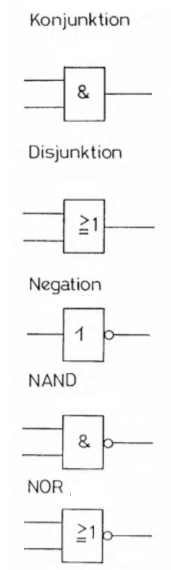
\includegraphics[height=0.8\textwidth]{logic_symbols}%
  \caption{Logic circuit symbols}%
  \label{fig:logic_symbols}
\end{figure}
Once drawn, such a circuit can look like this:

\begin{figure}[H]
\centering
  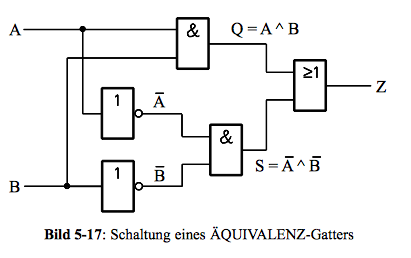
\includegraphics[height=0.3\textwidth]{equivalence}%
  \caption{Example for circuit design: the equivalence}%
  \label{fig:equivalence}
\end{figure}

\noindent
Now, before we set up this circuit, we have to think practical: Would it not be much more beautiful, and also much more easy, to just have one element instead of three different ones? In electronics, especially today in microelectronics (computers!), it is a key factor to build a circuit as easy as possible. Now, one can prove mathematically, that every circuit that is build up by OR's, AND's and Inversions, can also be build up by NAND's (negated AND) as well as by NOR's (negated OR). The circuit is shown again, but this time the elements were replaced by NAND's. 

\begin{figure}[H]
\centering
  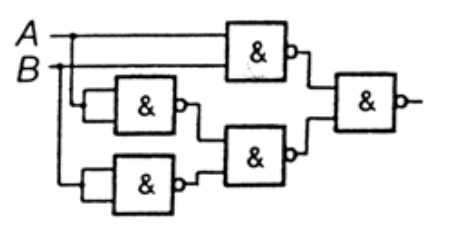
\includegraphics[height=0.2\textwidth]{equivalence_optimized}%
  \caption{Optimized equivalence circuit}%
  \label{fig:equivalence_optimized}
\end{figure}

So how do we actually replace the element with NAND's? To figure out the conversion, we compare the truth table of the NAND with that of different conminations of the three basic elements. We see, that a NAND with inverted output is a NAND (per definition) and an OR with inverted inputs is also a NAND. The conversions are seen below again. The clue is now, that if we insert anywhere two inverters after each other, it does not change the signal. After doing this, one can use the conversions below and end up with a circuit completely build up of NAND's. 

\begin{figure}[H]
\centering
  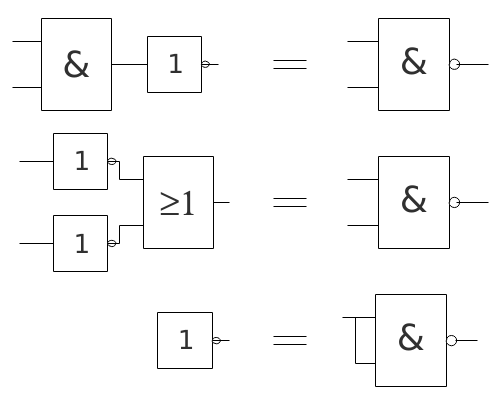
\includegraphics[height=0.33\textwidth]{nand_conversion}%
  \caption{Conversion to NAND}%
  \label{fig:nand_conversion}
\end{figure}

\section{Combinatoric circuits}
\subsection{General}
We differ between combinatoric circuits and sequential circuits. Combinatoric circuits are logical functions, whose \underline{output states are always exactly defined through their input variables}. This point will become more clear later when we look at sequential circuits. 

\subsection{Construction of a combinatoric circuit}
\begin{enumerate}
	\item Write down the truth table.
	\item Construct the disjunctive normal form from your truth table.
	\item Draw the circuit accordingly.
	\item Transform the circuit in such a way that it only uses NAND Gates.
	      How many NAND gates do you need? See if you can loose one or two gates.
	\item Check/discuss the circuit design again. An effective method is to create the truth table again just by looking at the circuit, then compare with what you should get. 
	\item If you're sure that your design works, build up the circuit with real components and connections. 
\end{enumerate}



%\subsubsection{Truth table}                            
%\subsubsection{Equation}                               
%\subsubsection{Draw circuit with logic elements}       
%\subsubsection{Unify}                                  
                                                       
\section{Sequential circuit}                           
\subsection{General}
Now we look at sequential circuits, which is different from the combinatoric circuit. Sequential circuits have something that can be looked at as a memory. The clue is, that the output of an operator is used again as one of the inputs. This means, that the circuit depends not only on combinatoric input variables, but also from the output of the step before. In this way, the functionality of a memory is realized. 

\subsection{Elements}
\subsubsection{Latch}
This concept is easily explained with the most basic realization of a sequential circuit. If the output has a default value of zero (this means, that there is no current on the output line in the beginning), then this zero-value also goes to one of the inputs. Now this stays as it is as long \texttt{A=0} as well. But now, if for once \texttt{A=1}, the OR-Operator will bring an output of \texttt{1}. Now, even if \texttt{A=0} again, will the output stay on \texttt{1}. We can say, that we saved the binary number \texttt{1}.

\begin{figure}[H]
\centering
  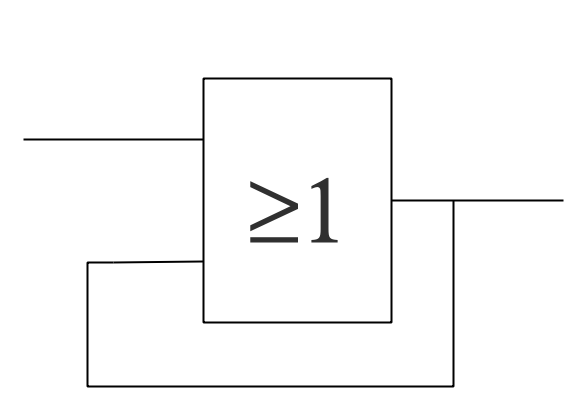
\includegraphics[height=0.2\textwidth]{loop}%
  \caption{Latch}%
  \label{fig:loop}
\end{figure}

\noindent
Of course, this is not very sophisticated yet, we cannot remove the output again or save something else. If we want a circuit that can set and reset a variable, we need a so called Flip-Flop. A diagram of a Set-Reset-Flip-Flop is shown below. One can see, that the output of the first OR-operator is fed back to the second OR-operator and vice versa. Now we can set and reset a variable, which gives us a memory function. It takes a bit of thinking to figure out what's going on exactly, which we are going to do later when we are going to build a sequential circuit. 

\begin{figure}[H]
\centering
  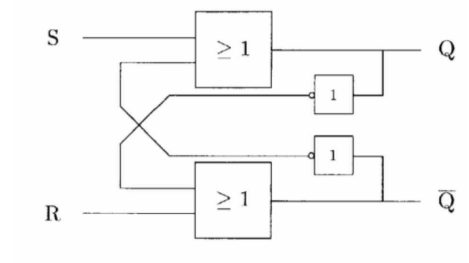
\includegraphics[height=0.35\textwidth]{RSFF}%
  \caption{RS-Flip-Flop}%
  \label{fig:RSFF}
\end{figure}

\subsubsection{Clock}
Because now we have the time as an additional dimension in our circuits, it is important to know, what exactly happens when. To control this, often a clock (Takt) is implemented. For this, we connect an additional variable (1 or 0) over an AND-operator with the input variables. If the clock is set to zero, the circuit is blocked and nothing can come in. If it is set to one, the circuit is open an may work as designed. The clue is now, to time the clock variable such, that it opens the circuit every time again, when the previous computation is over and the output ready for the next step. Another approach will be, that the circuit is designed in a way, that it is by construction blocked until the computation is over.

\begin{figure}[H]
\centering
  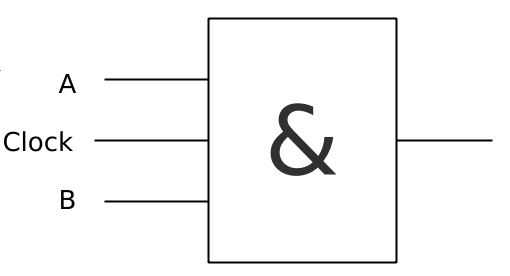
\includegraphics[height=0.2\textwidth]{clock}%
  \caption{Realization of a clock}%
  \label{fig:clock}
\end{figure}
\subsection{Construction of a sequential circuit}
